\documentclass[%
oneside,                 % oneside: electronic viewing, twoside: printing
final,                   % draft: marks overfull hboxes, figures with paths
10pt]{article}

\listfiles               %  print all files needed to compile this document

\usepackage{relsize,makeidx,color,setspace,amsmath,amsfonts,amssymb}
\usepackage[table]{xcolor}
\usepackage{bm,ltablex,microtype}
\usepackage{float}
\usepackage[pdftex]{graphicx}

\usepackage{graphicx}

\usepackage{fancyvrb} % packages needed for verbatim environments

\usepackage[T1]{fontenc}
%\usepackage[latin1]{inputenc}
\usepackage{ucs}
\usepackage[utf8x]{inputenc}

\usepackage{lmodern}         % Latin Modern fonts derived from Computer Modern

% Hyperlinks in PDF:
\definecolor{linkcolor}{rgb}{0,0,0.4}
\usepackage{hyperref}
\hypersetup{
    breaklinks=true,
    colorlinks=true,
    linkcolor=linkcolor,
    urlcolor=linkcolor,
    citecolor=black,
    filecolor=black,
    %filecolor=blue,
    pdfmenubar=true,
    pdftoolbar=true,
    bookmarksdepth=3   % Uncomment (and tweak) for PDF bookmarks with more levels than the TOC
    }
%\hyperbaseurl{}   % hyperlinks are relative to this root

\setcounter{tocdepth}{2}  % levels in table of contents

% --- fancyhdr package for fancy headers ---
\usepackage{fancyhdr}
\fancyhf{} % sets both header and footer to nothing
\renewcommand{\headrulewidth}{0pt}
\fancyfoot[LE,RO]{\thepage}
% Ensure copyright on titlepage (article style) and chapter pages (book style)
\fancypagestyle{plain}{
  \fancyhf{}
  \fancyfoot[C]{{\footnotesize \copyright\ 1999-2017, "Computational Physics I FYS3150/FYS4150":"http://www.uio.no/studier/emner/matnat/fys/FYS3150/index-eng.html". Released under CC Attribution-NonCommercial 4.0 license}}
%  \renewcommand{\footrulewidth}{0mm}
  \renewcommand{\headrulewidth}{0mm}
}
% Ensure copyright on titlepages with \thispagestyle{empty}
\fancypagestyle{empty}{
  \fancyhf{}
  \fancyfoot[C]{{\footnotesize \copyright\ 1999-2017, "Computational Physics I FYS3150/FYS4150":"http://www.uio.no/studier/emner/matnat/fys/FYS3150/index-eng.html". Released under CC Attribution-NonCommercial 4.0 license}}
  \renewcommand{\footrulewidth}{0mm}
  \renewcommand{\headrulewidth}{0mm}
}

\pagestyle{fancy}


% prevent orhpans and widows
\clubpenalty = 10000
\widowpenalty = 10000

% --- end of standard preamble for documents ---


% insert custom LaTeX commands...

\raggedbottom
\makeindex
\usepackage[totoc]{idxlayout}   % for index in the toc
\usepackage[nottoc]{tocbibind}  % for references/bibliography in the toc

%-------------------- end preamble ----------------------

\begin{document}

% matching end for #ifdef PREAMBLE

\newcommand{\exercisesection}[1]{\subsection*{#1}}


% ------------------- main content ----------------------



% ----------------- title -------------------------

\thispagestyle{empty}

\begin{center}
{\LARGE\bf
\begin{spacing}{1.25}
Project 1
\end{spacing}
}
\end{center}

% ----------------- author(s) -------------------------

\begin{center}
{\bf \href{{https://github.com/stiandb/compfys}}{FYS3150/FYS4150 - Hannah Berg, Stian Bilek \& Frida Furmyr}}
\end{center}

%    \begin{center}
%% List of all institutions:
%\centerline{{\small Department of Physics, University of Oslo, Norway}}
%\end{center}
    
% ----------------- end author(s) -------------------------

% --- begin date ---
\begin{center}
\today
\end{center}
% --- end date ---

\vspace{1cm}
\begin{abstract}
    
\end{abstract}

\newpage

\section{Introduction}

\newpage

\section{Method}

\newpage

\section{Code/Implementations}

\newpage

\begin{figure}[h]
\begin{center}
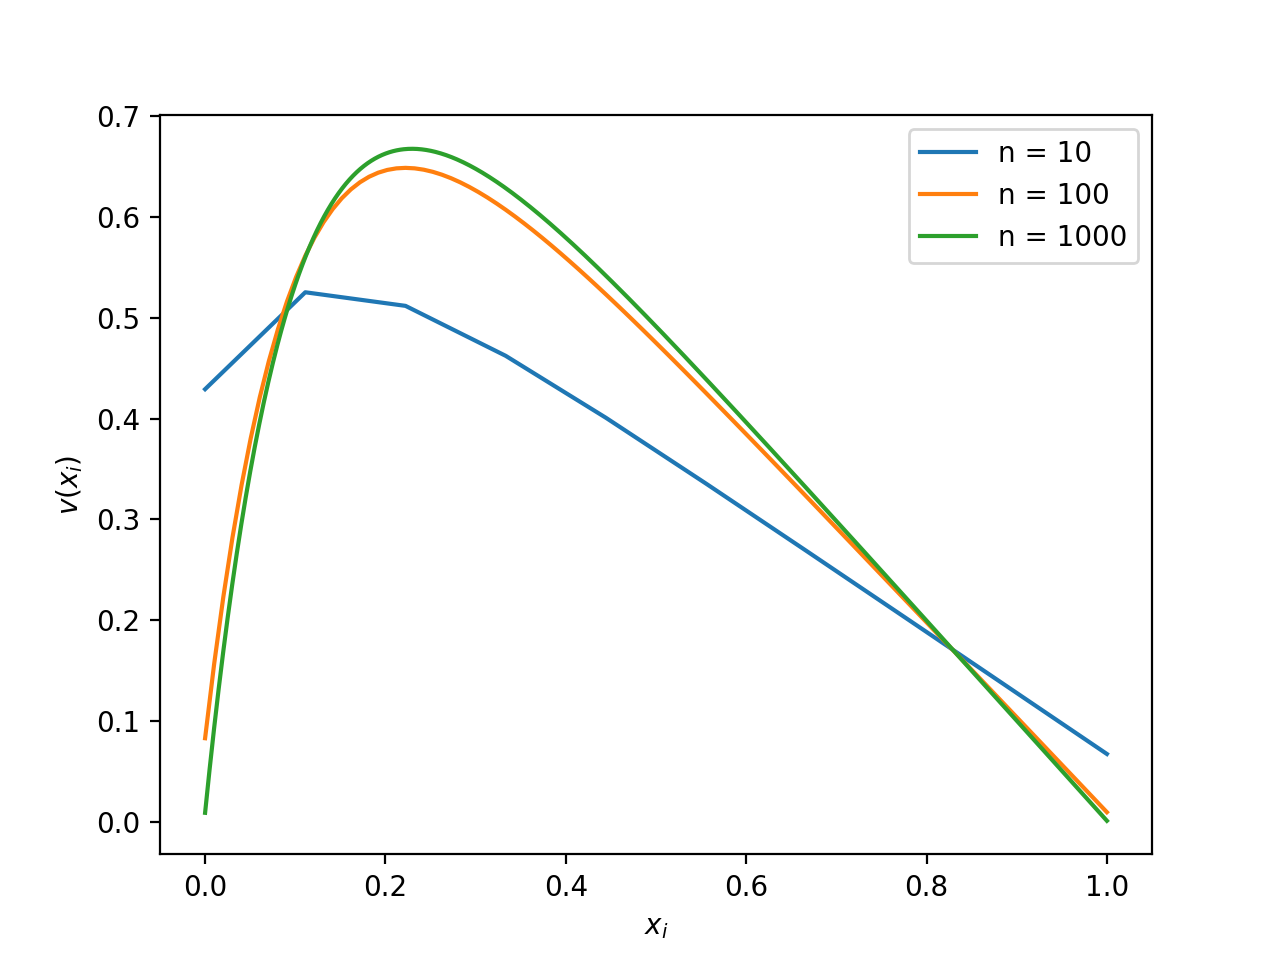
\includegraphics[width=12cm,height=10cm]{pro1.png}
\caption{Here is the solution to the set of linear equations.}
\label{Serie}
\end{center}
\end{figure}


Time $t$ to complete $n$ iterations

\begin{center}
    \begin{tabular}{| l | l | l | l |}
    \hline
    \textbf{iterations $n$} & \textbf{Gaussian Elimination $t$ (s)} & \textbf{Special Case $t$ (s)} & \textbf{Armadillo LU $t$ (s)} \\
    \hline
    $10^1$ & $2 \cdot 10^{-5}$ & $3 \cdot 10^{-6}$ & $2 \cdot 10^{-5}$ \\ 
    \hline
    $10^2$ & $2 \cdot 10^{-4} $ & $1 \cdot 10^{-5} $ &  $2 \cdot 10^{-4}$ \\
    \hline
    $10^3$ & $ 2 \cdot 10^{-4} $ & $9 \cdot 10^{-5}$ & $1 \cdot 10^{-2} $ \\
    \hline
    $10^4$ & $ 2 \cdot 10^{-3} $ & $8 \cdot 10^{-4} $ & $ 7 \cdot 10^{-0}$ \\
    \hline
    $10^5$ & $ 1 \cdot 10^{-2} $ & $ 5 \cdot 10^{-3}$ &  \\
    \hline
    $10^6$ & $2 \cdot 10^{-1}$ & $6 \cdot 10^{-2}$ & \\
    \hline
    
    \end{tabular}
\end{center}


Maximal relative error $\epsilon_{max}$  in $n$ iterations:

\begin{center}
    \begin{tabular}{| l | l |}
    \hline
    \textbf{iterations $n$} & \textbf{Maximal relative error $\epsilon_{max}$} \\
    \hline
    $10^1$ & $2.4$ \\
    \hline
    $10^2$ & $2.04$ \\
    \hline
    $10^3$ & $2.004$ \\
    \hline
    $10^7$ & $2.0000005$ \\
    \hline
   
    
    \end{tabular}
\end{center}


\newpage

\section{Analysis/Results}

\newpage

\section{Conclusions} 

\newpage


\section{Referencing}

\newpage

\end{document}